

\section{Software}
Software is much more than pure source-code.
As addition to every program a proper documentation is expected, as well a "tidied up" source-code that can be maintained easily.
For this reason the process of software-development has to be planned in-depth accurately be documented.


\subsection{Proceeding}
By the time the project is finished there will be two software-components.\\
First, a recommender-library that is capable of handling product-data and generating recommendation for any user based on his preceding behaviour.
Second, a online-shop that presents products and provides recommendations for products the user might like, based on the recommender-library.
As programming language for implementing the recommender-library Python has been chosen.
A MVC-Framework called Django will be used to set up the online-shop.

\subsection{Documentation}
The theory of the code will be explained in a separate document with many examples to visualize the way the recommendation system works.
Additionally there will be a documentation based on python-sphinx which will be automatically generated out of source-code comments.


\subsection{Milestones}
The development of the recommender algorithm will be subdivided into stages.
These can be seen in figure~\ref{fig:softwaremilestones}.
Each of the steps has to be finished before the next can start.\\

\begin{figure}[h!]

    \centering

    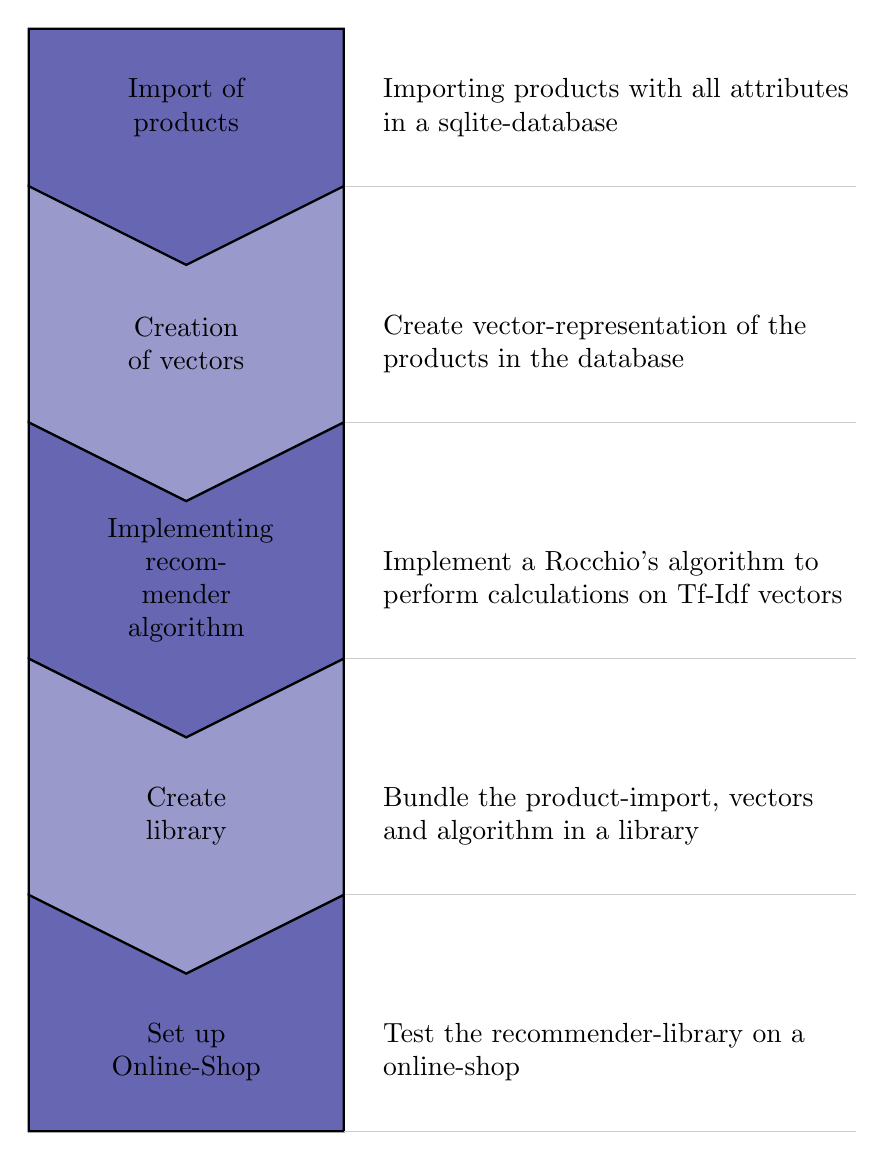
\begin{tikzpicture}

        \draw[thick,fill=Navy!60]
            (0,0)--(2,-1)--(4,0)--(4,2)--(0,2)--cycle;
        \node[text width=2cm,text centered,yshift=0] at (2,1) {Import of products};
        \node[text width=6cm,align=left,yshift=0] at (7.5,1) {Importing products with all attributes in a sqlite-database};
        \draw[thin,Black!20,yshift=0] (4,0)--(10.5,0);

        \draw[thick,fill=Navy!40,yshift=-3cm]
            (0,0)--(2,-1)--(4,0)--(4,3)--(2,2)--(0,3)--cycle;
        \node[text width=2cm,text centered,yshift=-3cm] at (2,1) {Creation of vectors};
        \node[text width=6cm,align=left,yshift=-3cm] at (7.5,1) {Create vector-representation of the products in the database};
        \draw[thin,Black!20,yshift=-3cm] (4,0)--(10.5,0);

        \draw[thick,fill=Navy!60,yshift=-6cm]
            (0,0)--(2,-1)--(4,0)--(4,3)--(2,2)--(0,3)--cycle;
        \node[text width=2cm,text centered,yshift=-6cm] at (2,1) {Implementing recommender algorithm};
        \node[text width=6cm,align=left,yshift=-6cm] at (7.5,1) {Implement a Rocchio's algorithm to perform calculations on Tf-Idf vectors};
        \draw[thin,Black!20,yshift=-6cm] (4,0)--(10.5,0);

        \draw[thick,fill=Navy!40,yshift=-9cm]
            (0,0)--(2,-1)--(4,0)--(4,3)--(2,2)--(0,3)--cycle;
        \node[text width=2cm,text centered,yshift=-9cm] at (2,1) {Create library};
        \node[text width=6cm,align=left,yshift=-9cm] at (7.5,1) {Bundle the product-import, vectors and algorithm in a library};
        \draw[thin,Black!20,yshift=-9cm] (4,0)--(10.5,0);

        \draw[thick,fill=Navy!60,yshift=-12cm]
            (0,0)--(4,0)--(4,3)--(2,2)--(0,3)--cycle;
        \node[text width=2cm,text centered,yshift=-12cm]at (2,1) {Set up Online-Shop};
        \node[text width=6cm,align=left,yshift=-12cm] at (7.5,1) {Test the recommender-library on a online-shop};
        \draw[thin,Black!20,yshift=-12cm] (4,0)--(10.5,0);

    \end{tikzpicture}

    \caption[Software Milestones]{software milestones}
    \label{fig:softwaremilestones}
\end{figure}


\FloatBarrier

\subsection{License}
If possible, the recommender library will be published under the MIT-License:\\

\begin{quote}
Copyright (c) 2015 \myAuthor

Permission is hereby granted, free of charge, to any person obtaining a copy of this software and associated documentation files (the "Software"), to deal in the Software without restriction, including without limitation the rights to use, copy, modify, merge, publish, distribute, sublicense, and/or sell copies of the Software, and to permit persons to whom the Software is furnished to do so, subject to the following conditions:

The above copyright notice and this permission notice shall be included in all copies or substantial portions of the Software.

THE SOFTWARE IS PROVIDED "AS IS", WITHOUT WARRANTY OF ANY KIND, EXPRESS OR IMPLIED, INCLUDING BUT NOT LIMITED TO THE WARRANTIES OF MERCHANTABILITY, FITNESS FOR A PARTICULAR PURPOSE AND NONINFRINGEMENT. IN NO EVENT SHALL THE AUTHORS OR COPYRIGHT HOLDERS BE LIABLE FOR ANY CLAIM, DAMAGES OR OTHER LIABILITY, WHETHER IN AN ACTION OF CONTRACT, TORT OR OTHERWISE, ARISING FROM, OUT OF OR IN CONNECTION WITH THE SOFTWARE OR THE USE OR OTHER DEALINGS IN THE SOFTWARE.
\end{quote}




